% Working draft for the EMSE 2026 Special Issue on Agentic SE.
% Author metadata, declarations, and the public artifact DOI remain open gates.
\documentclass[lineno,pdflatex,sn-basic]{sn-jnl}

\usepackage{graphicx}
\usepackage{amsmath,amssymb}
\usepackage{booktabs}
\usepackage{xurl}
\usepackage{placeins}
\raggedbottom
\setlength{\bibsep}{0.25em}

\begin{document}

\title[Participation Is Not Collaboration]{Participation Is Not Collaboration: Tracing Public Ownership After Cross-Product Agent Review}

\author*[1]{\fnm{Dao Sy Duy} \sur{Minh}}\email{Corresponding email pending}
\author[1]{\fnm{Huynh Trung} \sur{Kiet}}
\author[1]{\fnm{Tran Chi} \sur{Nguyen}}
\author[1]{\fnm{Pham Phu} \sur{Hoa}}
\author[1]{\fnm{Nguyen Lam Phu} \sur{Quy}}
\affil*[1]{\orgdiv{Affiliation pending}, \orgname{Institution pending},
  \orgaddress{\city{City pending}, \country{Country pending}}}

\abstract{\textbf{Context:} A pull request (PR) written by one coding-agent product and reviewed by another looks like a multi-agent workflow. Two products on one PR do not show that one addressed the other. \textbf{Objective:} We trace the public path from cross-product review to an addressed edge, a next owner, and a later state. \textbf{Method:} We screen 361,296 PRs in a pinned AIDev release and analyse 8,608 trigger PRs, 546 matched pairs, and a 1,067-PR outcome cohort. Exact account, comment, and review-batch identifiers anchor every event to one trigger. We set aside short automation bursts, match cross- to same-product triggers, trace earlier review history, and fix a check point at hour 48. \textbf{Results:} Direct dialogue between different products is rare. After a five-minute burst, user accounts own most remaining first actions, and most have reviewed in the repository before. Cross-product triggers get 13 percentage points less visible follow-up than matched same-product triggers. Among PRs still open at that point, an exact reply to the trigger is linked to 17 points more later merge. The link holds under stricter edge rules, a shuffle test inside each repository, and a whole-population model that drops the check point and lets the edge switch on in time. A user account writes that edge four times in five, so it marks human acknowledgement, not agent-to-agent dialogue. \textbf{Conclusions:} Public multi-agent impact should be reported as a map of connections, not as a count of products. Addressed edges and visible ownership are useful field signals, but they come from watching, not from an experiment.}

\keywords{coding agents, multi-agent software engineering, code review, human-agent collaboration, pull requests, mining software repositories}
\maketitle

\section{Introduction}\label{sec:introduction}

On a pull request today you can find two AI coding products at once. One writes
the change. A different one reviews it. It looks like two machines working as a
team, and it is easy to report it that way.

We followed what happens next, one event at a time. Almost none of it is
teamwork. The two products hardly ever answer each other. What we found instead
was a person. A maintainer reads the agent's review point and replies to it.
That reply is rare. It is also the one public connection that goes together with
the change being merged later. A count of products on a pull request measures
none of this.

The gap matters for research and for tool design. A short burst of bot events can
look like a conversation. A new review can be part of the same API call. A user
account can act next without having been chosen as a go-between. If these cases
are mixed together, a product count becomes a weak measure of teamwork.

Field studies already tell us a lot. They count agent-authored PRs, measure how
common AI review is, model reviewer order, and study how developers answer agent
comments \citep{li2026aidev,selvanayagam2026a2a,zhong2026agenticreview,
cynthia2026responses,khemissi2026references,duma2026reviews}. Several report that
people still carry the review \citep{zhong2026synergy,chowdhury2026industry}.
Designed systems show how known agents can pass messages, roles, files, or
structured disagreement
\citep{destefanis2026coordinate,qiu2026adversarial,zhang2026reporeviewer}.

What is still missing is a hard test. These studies count who appears, or they
read what was written. Neither tells us whether one actor actually answered
another. Our question is narrower and stricter: after one cross-product review
event, what connected public path can we point at in the data?

We ask three questions:

\begin{description}
\item[RQ1 -- Is there a handoff?] Once we split one review batch into its parts,
and set aside the fast burst of events that follows a trigger, does anything
left look like one product handing over to another? And who takes the next
visible step? The cost of handing a task between agents has been studied under
controlled interruptions \citep{kc2026handoff}. We ask the question that comes
before it: can a public handoff be seen at all?
\item[RQ2 -- Who bridges the boundary?] How much public follow-up happens across
the boundary between two products? And when a person steps in, have they worked
on this repository before?
\item[RQ3 -- Who writes the connection, and does it mark a later state?] Two
signals say that something connected: a reply pointing at the exact review
comment, and automation followed by a person. Does either go together with the
change being merged later, and who is it that writes the reply?
\end{description}

We make three contributions.

\textbf{An evidence ladder with a hard rung.} We separate four things that a
product count runs together: both products appearing on one PR, a reply that
points at the exact review comment, the next visible owner, and the later state
of the PR. The second rung is machine-checkable, and it is strict. It is what
makes the rest of the paper falsifiable.

\textbf{A finding that the ladder produces.} Each rung deletes most of what the
rung above admitted. Almost no cross-product activity becomes one product
answering another. The rare exact reply does mark a different later outcome, and
a person writes it four times in five. So the measurement choice changes the
conclusion, which is the point.

\textbf{A reusable check for order-based claims.} Reviewer order is often read as
evidence of coordination. We show that shuffling the order of events inside the
same PR reproduces the apparent pattern almost exactly. Prior work on review
order compares against an alphabetical baseline \citep{bouraffa2025orders}; we
argue a shuffled baseline is the one that can falsify a coordination claim.

We do not claim the first observation of AI-to-AI review. Full data rules, all
estimates, robustness checks, and rejected experiments are in Online Resource~1
(Supplementary Information).

\section{Related Work}\label{sec:related}

\subsection{Agent work in public repositories}

AIDev maps agent-authored work at GitHub scale \citep{li2026aidev}. Studies of
this and related data examine acceptance, failure, developer roles, merge
conflicts, review signals, and cross-PR references
\citep{pinna2026comparing,ehsani2026fail,cynthia2026roles,xu2026conflict,
nachuma2026review,khemissi2026references}. These studies make clear that
repository context and human participation matter. They also make merge a poor
stand-alone measure of an agent's quality.

Four lines of work sit closest to ours.

\emph{How common it is.} The nearest study counts same-product and
cross-product AI review, comment output, and speed of reply
\citep{selvanayagam2026a2a}. It reports that cross-product review is rare and
very fast. Our burst windows are a way of taking that speed seriously rather
than a new discovery.

\emph{Who reviews, and in what order.} Zhong et al. model ordered human, LLM,
and agent reviewer sequences across review eras \citep{zhong2026agenticreview}.
Bouraffa et al. ask whether the order of review activity is meaningful at all,
using an alphabetical baseline \citep{bouraffa2025orders}. Neither compares the
observed order against a shuffled one, which is the check we add.

\emph{Who does the work.} Several studies find that people still carry the
review. Zhong et al. report that developers adopt human suggestions far more
often than agent suggestions \citep{zhong2026synergy}. Chowdhury et al. report a
lower merge rate for PRs reviewed only by an agent than for PRs reviewed only by
people \citep{chowdhury2026industry}. Duma et al. report that most AI-generated
PRs get no review at all \citep{duma2026reviews}. Our RQ3 result agrees with the
direction of this work. What we add is a much stricter definition of what counts
as the human contribution, and a design that keeps it before the outcome.

\emph{Whether agent feedback helps.} Cynthia et al. study how developers respond
to individual agent review comments \citep{cynthia2026responses}, and Lin et al.
mine developer feedback to a deployed agentic reviewer
\citep{lin2026coderabbit}. Fatima et al. find that the quality of reviewer-bot
feedback shows no clear link to workflow outcomes \citep{fatima2026footprints}.
That null is worth holding next to our result: we do not measure whether a
review comment was good, only whether someone addressed it.

These papers occupy the broad claims that cross-product review exists, that
reviewer order matters, and that people answer agent feedback. Our unit is
different. It is one cross-product trigger, and the exact edges, batches,
owners, and later state that follow it.

\subsection{Designed multi-agent review}

Role-based systems such as ChatDev and MetaGPT make communication part of the
design \citep{qian2023chatdev,hong2023metagpt}. RepoReviewer divides review into
repository, file, priority, and summary roles \citep{zhang2026reporeviewer}.
Adversarial Review adds a critic that checks a review through structured
disagreement \citep{qiu2026adversarial}. SWE-Review tests a known
generate--review--revise loop \citep{wang2026swereview}. Controlled traces can
therefore reveal roles and messages directly.

Public GitHub traces are weaker but more natural. Product co-presence does not
prove shared memory, a joint plan, or private communication. We use
\emph{cross-product feedback} for the trigger and reserve \emph{public
coordination} for observable connections and ownership. This measurement
boundary is central to our novelty.

\section{Data and Method}\label{sec:method}

\subsection{Data and event anchor}

We pin AIDev-7.6M at revision
\nolinkurl{37bbe1533e26cc1e1374917dba1186d1c8a4dc81}. The release contains
7.69 million agent-authored PRs. We use the richer AIDev-pop layer: 361,296 PRs
from repositories with more than 100 stars. Its event tables contain submitted
reviews, inline review comments, PR comments, and selected lifecycle events.
PRs are created through 31 March 2026; we use 15 April 2026 at 00:00 UTC as the
common observation boundary.

We map only exact official GitHub identities to the six AIDev product labels.
Names that merely look similar are not guessed. The PR author carries one product
label. A \emph{trigger} is the first review, inline comment, or PR comment
written by a different product. We take the earliest such event on the PR, and it
must fall after the PR was opened and before it was closed. Everything we measure
afterwards is measured from the trigger. Online Resource~1 gives the full identity registry,
table coverage, joins, and denominators. Inline comments join to a submitted
review by review ID and then to the PR.

An \emph{addressed edge} means one thing only: a later comment points back at the
trigger comment itself, by identifier. It is the machine record that someone
answered this exact point, and nothing more. A reply somewhere else on the same
PR does not count. A later review must also carry a different review-batch ID.
These rules stop one API call from appearing to answer itself. Figure~\ref{fig:contract} shows the anchor, the
three exclusion rules, and the four evidence levels that the rest of the paper
keeps separate.

\begin{figure}[htbp]
\centering
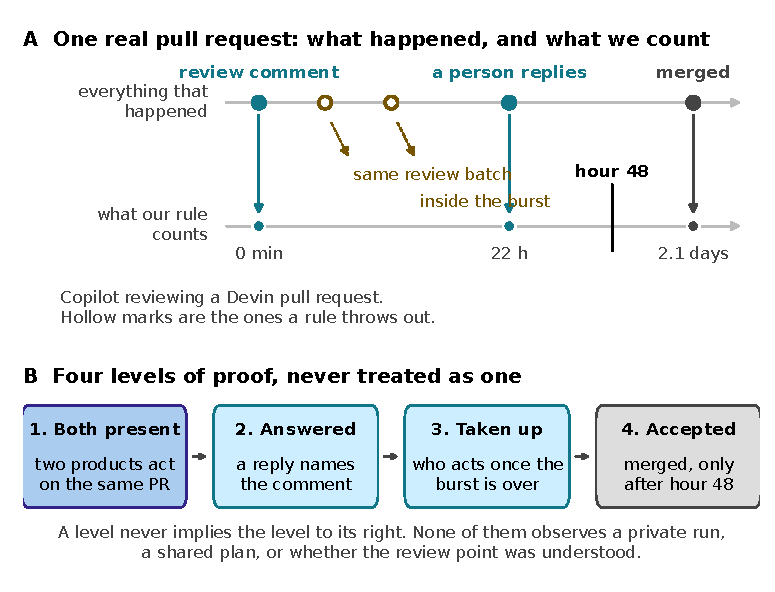
\includegraphics[width=\linewidth]{Fig1.pdf}
\caption{How we measure. Panel A puts one cross-product trigger on a single PR
and marks what each rule removes. A sibling comment in the same submitted review
batch is not a reply. An event inside the tested burst window does not define the
next owner. Only a comment whose parent identifier is the trigger's own
identifier counts as an addressed edge. The later state is read after a fixed
check point at hour 48. Panel B lists the four evidence levels in order. This is
a drawing, not data: the positions are for illustration only.}
\label{fig:contract}
\end{figure}

\subsection{Three analytic views}

A \emph{relay} means the next visible step is taken by a product different from
the one that wrote the trigger. It is the thing a multi-agent workflow would
produce, and it is what RQ1 looks for.

For RQ1, we follow each first cross-product trigger for seven days, ending at
PR closure when earlier. We join exact replies, new review rounds, later PR
comments, and visible force-push events. The first later owner is a user
account, mapped product, other bot, branch movement or untyped activity, or no
action. We repeat this state after excluding the first 0, 1, 5, 10, or 30
minutes. These windows test how much one fast automation burst is driving the
answer. They do not reveal a private run boundary. We then apply a second
five-minute waiting period, to test whether a mapped-product-first state really
becomes a relay to another product.

For RQ2 we build matched pairs. Each cross-product trigger is paired with a
same-product trigger from the same repository, the same PR-author account, the
same author product, the same source channel, and the same month. Pairing uses
nearest time without replacement.
We also identify the first distinct user account within 48 hours. Prior public
history requires that account to have submitted a review in the same repository
on a different PR strictly before the trigger.

For RQ3 we fix a check point at hour 48. We study only PRs that are still open
at that point, and we count merges only after it. This keeps cause before effect
in time. It is also a limit. Most cross-product inline-trigger PRs finish sooner,
so they fall outside the group, and we report how many with the results rather
than leaving it unsaid. The group also needs 30 complete days of later
observation. The exposure is an exact addressed
edge by hour 48; the outcome is merge after hour 48 and by day 30. A secondary
cohort classifies the first 48 hours as user first, automation then user,
automation without a user event, movement, other activity, or no action. This
lets us compare an automation-to-user relay with automation alone.

We report percentage-point contrasts because they are easy to read. Main
intervals cluster or resample by repository. Outcome models adjust for product,
channel or month where relevant, trigger age, and public activity known before
the trigger. We vary the addressed-edge window, add repository fixed effects,
and remove each product pair in turn.

The later-state comparison comes from watching, not from an experiment. So we
also ask how much hidden structure it would take to remove the result. We run
four checks.

First, an E-value \citep{vanderweele2017evalue}. It asks a simple question: how
strong would a cause we did not measure have to be, before it could wipe out our
result? A larger number means a more demanding requirement. Second, a grid that
shows how big one missing yes-or-no factor would have to be. Third, three
outcomes that had already finished before the trigger. The trigger cannot change
the past, so these should show no difference; if one of them does, that is a
warning sign and we report it as such. Fourth, a shuffle test that reassigns the
exposure label inside each repository.

We also run two checks that attack the design rather than the arithmetic. The
first drops the hour-48 rule and models the chance of merging over time across
the whole trigger population, with the edge switching on when it actually
happens. The second splits the edge by whether the person who wrote it had
already reviewed in that repository, and then repeats that split inside single
repositories.

These checks put a limit on fragility. They do not tell us what an intervention
would do. Task difficulty and maintainer intent are not measured here. Either
one could shape both the public path and the outcome.

\subsection{Reproducibility and AI use}

The artifact pins the data revision, stores PR-grain cohorts, generates all
tables and figures, and runs automated data and leakage checks. We also screened
current public review and agent-trace datasets against the same event contract.
A released AI-to-AI cohort checks product-pair and event-time attribution on
shared PRs. A full SWE-Review-Chat scan applies the exact identity, parent-edge,
overlap, and landmark rules. External rows are not pooled with the main cohort.
OpenAI Codex helped inspect data, write and test analysis code, search
literature, make figures, and edit the draft. The authors checked source
records, reran the analysis, verified cited sources, and reviewed the text and
figures. Human authors remain responsible for every claim, citation, and final
decision. No model is an author.

\section{Results}\label{sec:results}

\subsection{RQ1: product presence rarely becomes a relay}

Two products on one PR almost never becomes one product answering the other.
Once the fast automatic burst is set aside, a person usually takes the next
visible step.

Figure~\ref{fig:topology} gives two views of the same narrowing process, over
the complete seven-day cohort. Panel A shows how many PRs remain as the
connection rule gets stricter. Panel B shows the first visible owner after
each tested burst window, among PRs that still have an action. Later public
activity is common. An exact reply from a product different from the
triggering reviewer is not: it appears on fewer than 1\% of PRs. User accounts
write four in five of those exact replies.

\begin{figure}[htbp]
\centering
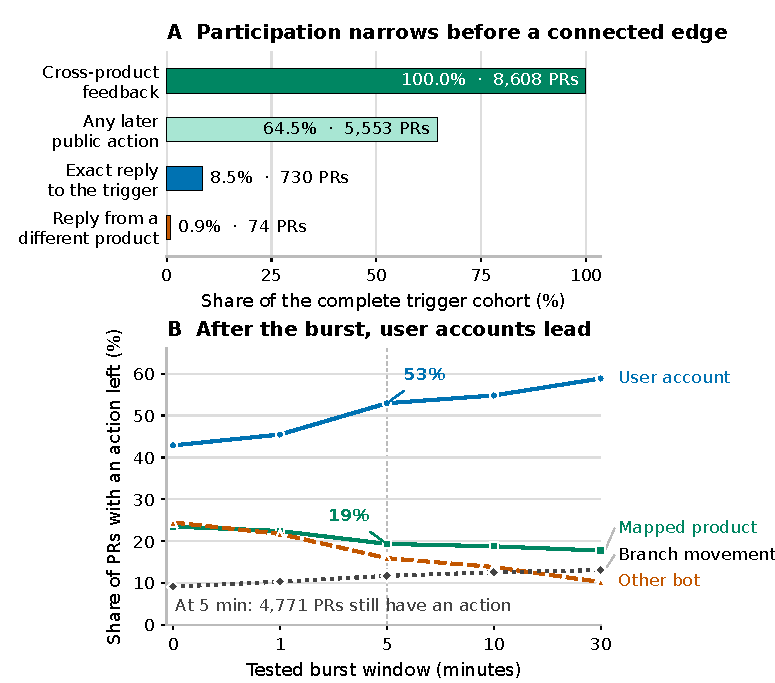
\includegraphics[width=\linewidth]{Fig2.pdf}
\caption{Public activity narrows before any connected edge appears. Panel A
shows the share and count of PRs that meet each stronger evidence rule; the full
cohort holds 8,608 PRs. Panel B shows the first visible owner after each of five
tested burst windows, among PRs that still have an action. At five minutes,
4,771 PRs still have one, and user accounts own 53\% of those actions against
19\% for mapped products. The windows are test settings, not known private run
boundaries.}
\label{fig:topology}
\end{figure}

The burst test changes the owner, not only the time. After five minutes,
mapped products lose close to a third of their mapped-first classifications.
User accounts then own far more of the remaining actions than mapped products
do. This ordering holds in every leave-one-repository-out and
leave-one-product-pair-out check.

The next step is even more selective. Among PRs that are still mapped-product
first after five minutes, only about one in twenty move next to a different
mapped product after a second waiting period.

The same product carrying on is far more common, and it is tempting to read
that as an agent staying with the task. It is not. We shuffled the order of
the later events inside each PR, keeping that PR's own mix of products, and
the shuffled data reproduce the pattern almost exactly. So the trace supports
one thing only: a relay to another product is rare. It gives no support for a
special product-persistence mechanism.

\noindent\textbf{Answer to RQ1.} Two products on one PR greatly overstates how much handing over really happens. Once the fast burst of events is set aside, user accounts are the main visible owner. A relay to another mapped product is rare.

\subsection{RQ2: familiar user accounts bridge a quiet boundary}

\begin{figure}[!htbp]
\centering
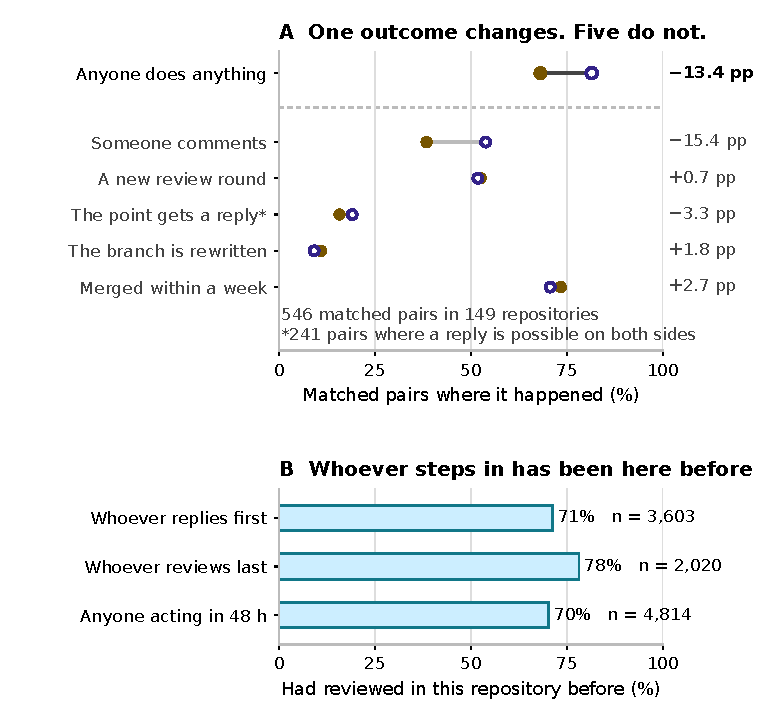
\includegraphics[width=\linewidth]{Fig3.pdf}
\caption{A quieter boundary, and a history that is common on both sides of it.
Panel A compares later public action for cross- and same-product triggers in
nearest-time matched pairs. Pairs share repository, author account, author
product, source, and month. The sample holds 546 pairs from 149 repositories,
with follow-up after 68.1\% of cross-product and 81.5\% of same-product
triggers; the gap is 13.4 points, 95\% interval $-19.9$ to $-4.0$ from
resampling repositories.
Panel B compares the first user bridge, the first later decisive reviewer, and
all users who answered within 48 hours. A decisive reviewer is one who approves
or asks for changes. History means a public review on another PR in the same
repository before the trigger. The open circle marks the wider responder
baseline. A past review does not tell us whether an account used a tool,
remembered the repository, worked by hand, or was picked on purpose.}
\label{fig:bridge}
\end{figure}

The cross-product boundary is a quieter one. Comparable triggers get less
visible follow-up across it, and when someone does step in, it is usually a
person who has reviewed in that repository before.

Visible follow-up is less common after a cross-product trigger than after its
matched same-product partner. The gap is 13.4 percentage points
(Figure~\ref{fig:bridge}A). No other outcome supports a claim that this
quieter boundary leads to more branch movement or more merges.

Figure~\ref{fig:bridge} joins the matched comparison with a wider history
check. Seven in ten of the first user-account bridges had already reviewed
another PR in that repository. That rate is close to the rate among all users
who answered within 48 hours. So prior history is common right across the
response layer. It does not tell us why one account rather than another
becomes the bridge.

\noindent\textbf{Answer to RQ2.} Comparable cross-product feedback has less
public follow-up. When a user account becomes the visible bridge, it is usually
not a repository newcomer, but the trace does not show deliberate expert
routing.

\FloatBarrier
\subsection{RQ3: a person writes the edge that marks a later state}

\begin{figure}[!htbp]
\centering
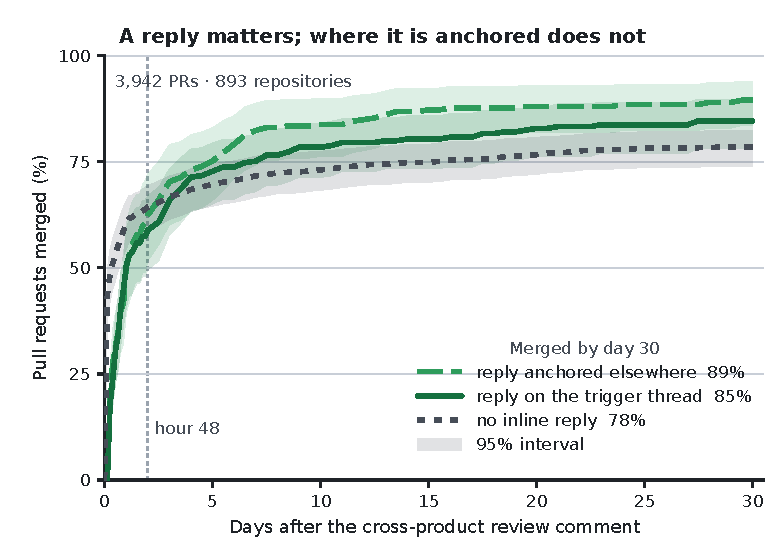
\includegraphics[width=\linewidth]{Fig4.pdf}
\caption{Connected public signals and later merge. Panel A shows raw later-merge
rates: 55\% with an exact edge, 41.7\% for other public discussion without one,
and 37.9\% across all PRs without one. The discussion group sits inside the
no-edge group. Panel B shows adjusted differences. The top three rows are the
same group of PRs under three rules for what counts as an edge: any exact parent
reply, the same edge after dropping replies written by the triggering product
itself, and edges written by a user account. The fourth row is the
discussion-only control. The fifth, marked with a diamond, is the separate
automation-to-user route, which has its own group and its own reference. Each row prints its estimate and 95\% interval. These are links in observed
data, not causes.}
\label{fig:relay}
\end{figure}

Among the slower PRs that are still open at hour 48, one signal stands out as
a marker of later merge: an exact reply to the trigger. Four times in five, a
person writes it.

The group holds 1,067 inline-trigger PRs. It is the slower-moving part of the
population. Most cross-product inline-trigger PRs close, and most of those
merge, at or before hour 48. Our group is the 27\% that are still open when
the outcome window opens. Everything below describes that slower group, not
the most common kind of cross-product PR.

The exposure also needs naming precisely. The rule is a reply whose parent
identifier is the trigger's own identifier. It does not require another
product to write that reply. Across the exposed reply events, user accounts write the large majority. The
triggering product replies to its own comment in a small number of cases, a few
more come from bots we do not map to a product, and only three come from a
mapped product other than the one that wrote the trigger. So the connected
signal here is a person acknowledging an agent's review point. It is not a
conversation between agents.

Later merge is more common when there is an exact reply to the trigger than
when there is none (Figure~\ref{fig:relay}A). After adjusting for what was
already visible before the trigger, the difference is 17.3 percentage points.
It stays positive for reply windows from one to 48 hours, in a model that only
compares PRs inside the same repository, and after removing each ordered
product pair in turn. We also tested it against a harder comparison. Instead of an edge versus
silence, we compared an exact edge with PRs that already carry other public
discussion. The result stays positive.

Because most exposed replies are written by people, we refit the model under
two stricter rules for what counts as an edge. One drops replies written by the
triggering product itself. The other keeps only replies from a user account.
Both give the same answer, with intervals that stay clear of zero
(Figure~\ref{fig:relay}B, rows two and three). The result is a property of the
addressed edge, not of a product answering itself. Only three PRs carry an exact reply from a mapped product other than the
trigger's. That is far too few to model. The count is the RQ1 finding showing up
again at the outcome stage.

The exact edge is not the only visible thing that goes with a later merge. A
wider model that puts all four post-trigger states side by side shows a small
group of PRs with branch movement and no discussion sitting even higher, on a
very wide interval. Any visible sign that a PR is still being worked on points
the same way. We report that model in Online Resource~1 and keep the harder
discussion-only comparison as our main specificity check.

The automation-to-user route gives a separate check on a wider group. It is
linked to 12.9 points more later merge than automation alone, after the same
kind of pre-trigger adjustment. Figure
\ref{fig:relay} first compares raw later-merge rates, including other public
discussion without an exact edge. Panel B shows two exact-edge comparisons and
the separate automation-to-user check. The diamond marks the row with a
different cohort and reference.

\begin{figure}[!htbp]
\centering
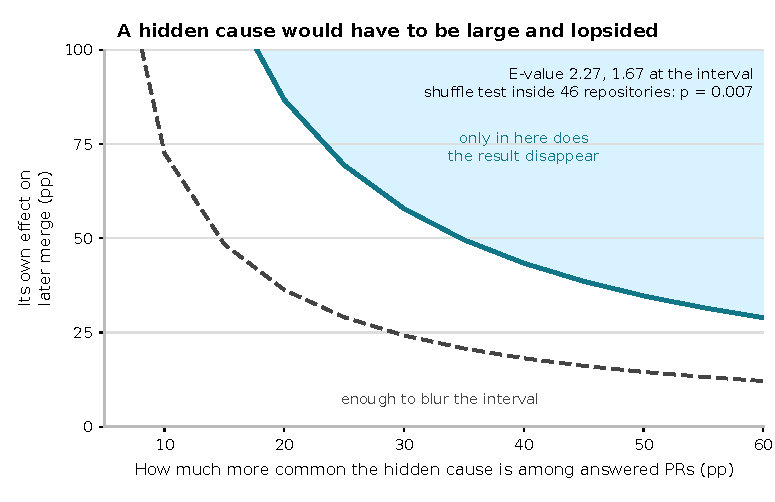
\includegraphics[width=\linewidth]{Fig5.pdf}
\caption{How much hidden structure it would take to remove the exact-edge
result. Panel A shows the arithmetic directly. One missing yes-or-no factor,
fixed before the trigger, removes the result only inside the shaded corner. To
get there it must be much more common among edge PRs \emph{and} carry a large
later-merge difference of its own. The dashed line is the weaker requirement
that removes only the interval. As a single summary, the E-value is 2.27, and
1.67 at the interval limit. Panel B applies the same adjusted model to three
outcomes that had already finished before the trigger, so the trigger cannot
produce them. The teal line marks the observed edge result for scale. Two of the three sit on
zero. Earlier user activity leans positive here and clears zero at a one-hour
reply window, so the text reports its estimate rather than treating it as a
pass. These are limits on fragility, not evidence of cause.}
\label{fig:sensitivity}
\end{figure}

Figure~\ref{fig:sensitivity} asks how fragile that result is. The E-value here
is 2.27. A hidden cause would have to be tied to both the exact edge and to
later merge by at least that much, on top of every control we already measure,
before it could explain the result away. Panel~A shows the same idea as a
grid. The shaded corner is where such a factor would have to sit, and it is a
demanding corner.

A shuffle test gives a second check, one that rests on the design rather than
on a formula. We keep only repositories that hold both kinds of PR. Inside each
one we shuffle the exposure label many times and refit. The shuffled results
centre on zero, and the real result sits far out in the tail ($p=0.007$,
two-sided). So the finding does not rest on the standard interval formula.

The three before-the-fact outcomes are the weakest of these checks, so we
report them as estimates rather than as a verdict. Two of them, an earlier
decisive review and earlier branch movement, sit close to zero at every reply
window. The third does not. Earlier user activity is $+7.0$ points at the
48-hour window, with a 95\% interval of $-1.7$ to $15.7$. At one hour it is
$+16.7$ points, and that interval clears zero. The one-hour value is a plain
failure, and it is why 48 hours is our main window. The 48-hour value is a
small leftover, based on too few PRs to be sure. It points in exactly the
direction a doubtful reader would expect, so we report it as an estimate and
not as a clean zero.

Two further checks matter more than any of the bounds above, because they
attack the design rather than the arithmetic.

\begin{figure}[!htbp]
\centering
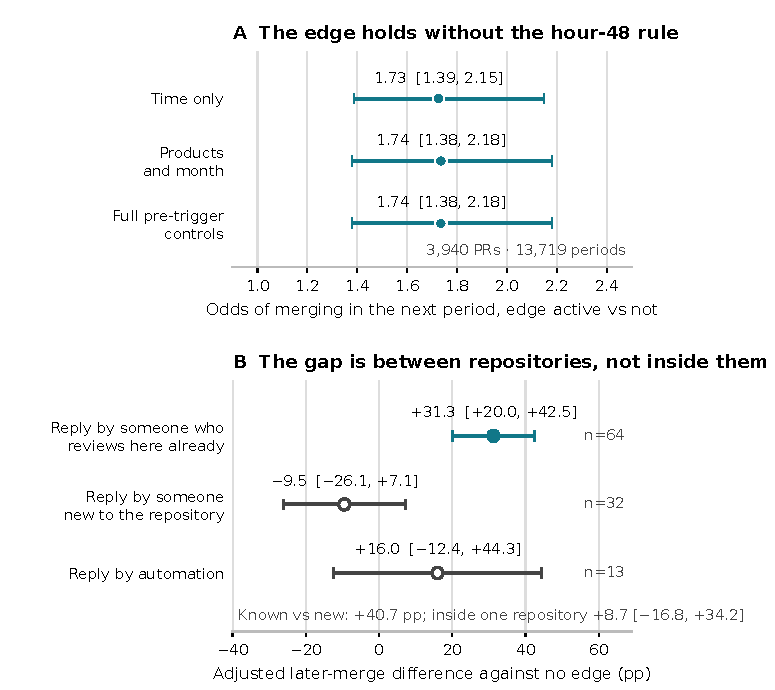
\includegraphics[width=\linewidth]{Fig6.pdf}
\caption{Two harder tests of the same result. Panel A drops the hour-48 rule
entirely. It follows every cross-product inline-trigger PR from its trigger and
asks how the chance of merging in the next stretch of time changes once an exact
reply exists. A PR counts as unexposed until its own reply arrives, so no time
before the reply is credited to it. Panel B splits the edge by who wrote it,
against PRs with no edge. The gap between a familiar replier and a newcomer is
large, but it nearly disappears when the comparison is held inside one
repository, so the trace cannot separate the person from the project.}
\label{fig:extensions}
\end{figure}

The first drops the hour-48 rule. Instead of keeping only PRs that are still
open, we follow every cross-product inline-trigger PR from its trigger and ask
how the chance of merging in the next stretch of time changes once an exact
reply exists. A PR counts as unexposed until its own reply arrives. The odds of
merging are about $1.7$ times higher while an edge is active
(Figure~\ref{fig:extensions}A), and the value barely moves as controls are
added. So the result is not an artefact of studying only slower PRs.

The second asks who wrote the edge. We split the exposed PRs by whether the
replier had already reviewed in that repository before the trigger. Almost all
of the association sits with the familiar repliers. A reply from someone new to
the repository shows no positive link at all (Figure~\ref{fig:extensions}B).
That looks like a mechanism, and we were tempted to report it as one. It does
not survive the obvious check. When the comparison is held inside a single
repository, the gap between the two kinds of replier shrinks to near zero with
an interval that spans it. Familiar repliers and newcomers are mostly in
\emph{different repositories}, and those repositories differ in how often
anything gets merged. We therefore report the split as a description of where
the signal sits, not as evidence that knowing the repository is what makes the
reply work.

An exact reply may mark a clearer issue, an engaged maintainer, a useful
comment, or another unmeasured condition. The data do not tell us which. The
result supports the value of a connected trace as a field signal; it does not
show that adding a reply would cause a merge.

\noindent\textbf{Answer to RQ3.} A person writes the connection, and the
connection marks a later state. The exact addressed edge survives every check we
ran, including dropping the hour-48 rule and letting the edge switch on in time.
Four times in five it is written by a user account rather than by an agent.
Nearly all of its association sits with repliers who already review in that
repository, but that split is between repositories rather than inside them, so
we cannot show that familiarity is the reason. Nothing here is causal.

\FloatBarrier
\section{Discussion}\label{sec:discussion}

\subsection{What this changes}

The picture a product count paints is wrong in a specific way. It shows two
agents in conversation. The trace shows something else: a thin map in which the
agents rarely speak to each other, and in which the connection that matters is
a person answering an agent. That person is usually not new to the repository.
Their reply is rare, it is easy to record, and it is the one public signal in
our data that goes together with the change being merged later. This is a link
we observed, not a cause we proved. But it points at a different thing to build
and a different thing to measure.

We also tried, and failed, to name the mechanism. Splitting the edge by whether
the replier already reviews in that repository produces a very large gap. Held
inside one repository, the gap goes away. The honest reading is that our signal
is a composite: it marks a project where people answer review points and PRs get
merged, and the trace cannot pull the person and the project apart. That is a
limit worth stating plainly, because a reader who saw only the split would draw
a stronger conclusion than the data support.

Prior work has shown that several reviewer types can appear in one PR, and that
their order can relate to review outcomes. Our narrower result explains what
that order hides. One review batch can create several events. A short burst can
look like a handoff. A product that seems to keep going may just reflect which
products are installed. And once a person takes over, the work can bounce back
to either product. Exact identifiers let us tell these paths apart.

The main field pattern is therefore not a self-running team. It is a thin map of who takes over next. Different-product dialogue is rare, user accounts often
bridge the visible boundary, and the most concrete edge is linked to a
different later state. This event-level view links natural repository data to the explicit message graphs used in designed multi-agent systems.

\subsection{Implications for agentic software engineering}

\textbf{Record the edge, not only the actors.} Review platforms and the
platforms that run agents should store four things: what a message replies to,
the review-batch ID, the run or session ID, and who is expected to act next. A
timestamp on its own cannot separate a burst of parallel events from a real
handoff.

\textbf{Make ownership transfer visible.} A product should be able to mark a
review point as received, declined, routed, or awaiting a user. This would turn
an inferred event sequence into an auditable coordination contract. The rare
different-product relay shows that co-installation alone does not provide this
contract.

\textbf{Use connected signals to guide tests, not as success scores.} The exact
edge is a promising marker for checking work, because it is clear and stable.
But it is rare. Only 8.5\% of trigger PRs carry one, and about one in ten PRs
in the hour-48 group do. It rarely fires by mistake, which makes it
useful for auditing. It is not a score, and not yet a quality metric. A prospective study should randomize an
explicit acknowledgement or routing feature and then measure resolution,
rework, review time, and merge.

\textbf{Support repository-aware human bridges carefully.} Visible user
bridges often have prior review history, so systems can offer context from past
reviews when asking for help. However, the high baseline among all responders
means history should not be sold as proof of expert selection.

\subsection{Trying to prove ourselves wrong shaped the story}

Several attractive claims did not survive stronger checks. A product that
appeared to keep going was matched by a random-order shuffle of the same PR's
own events. The newest example is the one above: repository familiarity looked
like the reason the edge works, until the comparison was held inside a single
repository. Repeated automation
did not show a special escalation dose. Post-burst ownership moved in both
directions rather than showing one-way user takeover. Prior review history did
not support a stable within-repository merge advantage. Request events lacked
the target identity needed to prove deliberate routing. Structural comment
overlap also remains semantically uncoded. We keep these results and all gates
in Online Resource~1 rather than turning them into positive
headlines. We also ran the same rules over a large review dataset packaged by other people.
After removing the PRs that overlap ours, it left no separate group of
exact-edge PRs at the hour-48 check point. That is a failed replication gate,
not proof that such edges never occur. It shows why being in the same thread
cannot replace a reply that points at the exact comment.

\section{Threats to Validity}\label{sec:threats}

\textbf{What we can see.} The event tables do not cover the same PRs. A missing
row can mean there was no event, or that the event was not captured. Ordinary
commit and review timeline rows carry no usable time in this release. So we
make claims about timing only for event types that do carry a usable time. We
also treat a force-push as branch movement, not as a checked fix.

\textbf{Identity and meaning.} Our list of approved accounts is strict, so it
may miss some agent accounts. A GitHub \texttt{User} account does not prove that
a person worked alone. An exact parent link proves that someone addressed the
point. It does not prove understanding, agreement, or repair. We never see
private messages, prompts, or shared memory.

\textbf{Which PRs we kept.} The hour-48 check point keeps only PRs that are
still open at that moment, and most cross-product inline-trigger PRs close before
then. The landmark numbers therefore describe slower PRs. The whole-population
model in Figure~\ref{fig:extensions}A is our answer to this: it uses every
trigger PR, and it still finds the same direction. Shorter reply windows raise a
further problem, because a reply inside such a window could itself change whether
the PR is still open at hour 48. We treat those windows as extra checks only, and
the 48-hour window is the main one.

\textbf{What the edge means.} An exact parent edge records that someone
addressed the trigger. It does not record who. In this group that someone is
almost always a user account, so RQ3 measures a person acknowledging an agent,
not one product handing over to another.

We also rely on the parent identifier that GitHub exports with each inline
comment. That field may point at the first comment in a reply thread rather
than at the comment just before. If so, our edge means ``in a thread that
starts at the trigger'', which is a looser idea. It would not change the RQ1
ordering, but it would make the measure looser.

\textbf{Selection and cause.} Matching holds several visible factors fixed, and
the outcome models use pre-trigger controls and repository-aware intervals.
They cannot balance what a review meant, how hard the task was, what the
maintainer intended, or what happened in private.

The stress test puts a limit on this. A hidden cause weaker than an E-value of
2.27 cannot account for the edge result. A stronger one still could. And the
before-the-fact user-activity check shows that selection of this kind is
present in our data, and only partly measured. Our controls also include no
stand-in for task difficulty. The later-state findings stay associations.

\textbf{How far the results reach.} AIDev-pop covers public repositories with
more than 100 stars, and the product pairs are uneven. Leave-one-out checks
ease the worry that a few repositories or a few pairs drive the result. They do
not extend it to private projects or to future versions of these products. The
outside dataset we screened checks our schema and identities, but after
removing overlap it gives no independent group for RQ3.

\section{Conclusion}\label{sec:conclusion}

Two AI products on one pull request is not proof of teamwork. Once the fast
burst of events is set aside, product co-presence almost never becomes one
product answering another. User accounts form the main visible bridge, and most
of them have reviewed in that repository before.

The clearest connected signal is an exact reply to the trigger. It marks more
later merges, and it survives stricter edge rules, a shuffle test, and a model
that drops the hour-48 rule and uses the whole population. A person writes that
signal four times in five. So the edge that
carries the weight is a human answering an agent, and that is exactly what a
count of products does not measure. Field evaluation of multi-agent work should
ask for three things: an addressed edge, a visible owner, and a later state.

\section*{Statements and Declarations}

\textbf{Funding:} Pending author confirmation.\quad
\textbf{Competing interests:} Pending author confirmation.\quad
\textbf{Data availability:} The source data are the public AIDev-7.6M
release at the pinned revision reported in Section~\ref{sec:method}. The
derived cohorts needed to reproduce the results will be archived at
[ARTIFACT DOI PENDING].\quad
\textbf{Code availability:} Analysis and figure code will be archived with the
derived cohorts at [ARTIFACT DOI PENDING].\quad
\textbf{Ethics approval:} Final institutional wording is pending author
confirmation for this public repository trace study.\quad
\textbf{Consent to participate:} Pending author confirmation.\quad
\textbf{Consent for publication:} Pending author confirmation.\quad
\textbf{Author contributions:} Pending author confirmation.

\bibliography{references}

\end{document}
